\documentclass[conference]{IEEEtran}
\IEEEoverridecommandlockouts
\usepackage{cite}
\usepackage{amsmath,amssymb,amsfonts}
\usepackage{algorithmic}
\usepackage{graphicx}
\usepackage{subcaption}
\usepackage{textcomp}
\usepackage{xcolor}
\usepackage{tikz}
\usepackage{multirow}
\usepackage{booktabs}
\usepackage{array}
\usepackage{float}
\usepackage{hyperref}
\usepackage{url}
\usetikzlibrary{positioning}

\def\BibTeX{{\rm B\kern-.05em{\sc i\kern-.025em b}\kern-.08em
    T\kern-.1667em\lower.7ex\hbox{E}\kern-.125emX}}
\begin{document}

\title{Solving the N-Queens Problem with Exhaustive Search and Metaheuristic Optimization\\
}

\author{\IEEEauthorblockN{Yash B.}
\IEEEauthorblockA{\textit{Department of Business} \\
\textit{AI Research Group}\\
\textit{Univ. of Europe for Applied Sciences}\\
Konrad-Ruse Ring 11, 14469 Potsdam, Germany. \\
student details to be updated}
\and
\IEEEauthorblockN{Raja Hashim Ali}
\IEEEauthorblockA{\textit{Department of Business} \\
\textit{AI Research Group}\\
\textit{Univ. of Europe for Applied Sciences}\\
Konrad-Ruse Ring 11, 14469 Potsdam, Germany. \\
hashim.ali@ue-germany.de}
}

\maketitle

\begin{abstract}
The N-Queens problem is a classical benchmark for studying exact search, local search, and population-based optimization in artificial intelligence because it combines simple rules with rapidly growing combinatorial complexity. It remains important for evaluating how optimization strategies behave when the search space becomes very large and when exact reasoning becomes increasingly expensive. A common gap in educational implementations is that algorithms are often demonstrated independently without a unified benchmarking pipeline that records runtime, memory, structured outputs, and visual evidence across several board sizes. This project addresses that gap by implementing depth-first search, greedy hill climbing, simulated annealing, and a genetic algorithm inside a notebook-based evaluation workflow for board sizes 10, 30, 50, 100, 200, and 500. The results show that exhaustive depth-first search is reliable only for the smallest case, while the three heuristic and metaheuristic approaches solve all tested larger cases with much better scalability. Greedy search achieved the strongest time efficiency, simulated annealing provided stable performance, and the genetic algorithm remained effective but computationally heavier. These findings demonstrate a practical comparison framework and show how different optimization paradigms trade completeness, speed, and memory efficiency.
\end{abstract}

\begin{IEEEkeywords}
N-queens problem, optimization algorithms, genetic algorithm, exhaustive search technique, local search techniques
\end{IEEEkeywords}

% \section{General instructions}
% Comment out this section after completing your write up.
% \begin{enumerate}
% \item You must have exactly the mentioned sections with the mentioned number of paragraphs.
% \item DO NOT DELETE ANY TEXT FROM THIS REPORT. JUST COMMENT OUT AND WRITE THE RELEVANT TEXT UNDER EACH COMMENT.
% \item Observe the report page limits (minimum 5 pages without references) and limit on maximum text is 7 pages without references.
% \item In case of figures, keep your raw data table also stored as excel file in this repository.
% \item Each paragraph must consist of 7-10 sentences.
% \item Add references where required.
% \item Total references should be between 10 and 15.
% \item Use latest references with 80\% references later than 2020.
% \item Use Google scholar for finding references and not Google or any other source.
% \end{enumerate}

\section{Introduction}
Optimization strategies are central to smart systems because they help agents choose high-quality actions under limited time, limited memory, and expanding search spaces. In intelligent systems, the choice of optimization strategy strongly affects whether a problem can be solved exactly, approximately, or not at all within practical computational budgets. Search-driven optimization is used in scheduling, planning, resource allocation, routing, and decision support, where solution quality and scalability must be balanced carefully \cite{russell2021aima,benaissa2024metaheuristic,houssein2024metaheuristics}. Exact algorithms are often preferred when guarantees are essential, but heuristic and metaheuristic methods become more attractive when the search space grows too rapidly. Recent reviews also emphasize that algorithm selection should be based on the exploration--exploitation tradeoff, scalability, and representation choices rather than on raw popularity alone \cite{rashed2024advancements,ruiztorrubiano2025mdp}. For that reason, benchmark problems with interpretable constraints remain useful in applied AI education and research. The N-Queens problem provides one such benchmark because it is easy to describe but difficult to scale. It therefore offers a compact environment for comparing exhaustive and non-exhaustive optimization behaviour side by side.

The importance of optimization algorithms for the N-Queens problem comes from the fact that the number of possible placements increases explosively as the board grows. Even though the constraints are simple, namely no two queens may share the same row, column, or diagonal, the search space quickly becomes challenging for classical exhaustive methods. This makes N-Queens a useful testbed for studying backtracking, conflict minimization, probabilistic search, and evolutionary improvement \cite{minton1992minconflicts,kirkpatrick1983optimization,jain2023efficient}. In this project, four approaches were implemented and benchmarked uniformly: exhaustive depth-first search, local greedy search, simulated annealing, and a genetic algorithm. The report focuses on how these approaches differ in runtime, memory, and practical solvability for board sizes from 10 to 500. The experimental notebooks also export structured CSV files and figures so that analysis is reproducible and presentation-ready. This unified workflow strengthens the value of the benchmark because the methods are compared under the same output and visualization pipeline. As a result, the study does not only solve N-Queens instances, but also demonstrates which optimization strategies remain useful as instance size grows.

\subsection{Related Work}
Research on the N-Queens problem and related optimization strategies covers exhaustive search, local search, simulated annealing, evolutionary methods, and recent broader optimization reviews. Classical work established that min-conflicts can outperform traditional backtracking by several orders of magnitude on large constraint satisfaction instances \cite{minton1992minconflicts}. Modern AI texts still use N-Queens to illustrate the difference between exact and heuristic reasoning in search-heavy environments \cite{russell2021aima}. Recent surveys on metaheuristic optimization have also highlighted the importance of balancing exploration and exploitation when choosing between hill climbing, annealing, and evolutionary search \cite{benaissa2024metaheuristic,houssein2024metaheuristics,salgotra2024systematic,rashed2024advancements}. N-Queens-specific literature also continues to evolve, including practical code-oriented implementations \cite{jain2023efficient}, higher-dimensional formulations \cite{kunt2024higher}, and improved local-search or hybrid metaheuristic approaches \cite{hussein2024nmra}. In this report, the related work is summarized to position the current implementation as a structured comparative study rather than as an isolated algorithm demonstration. Table~\ref{tab:LiteratureSummary} summarizes representative literature that informed the design choices for the present work.

\begin{table*}[!ht]
\centering
\caption{Literature review summary for search and optimization methods relevant to the N-Queens problem.}
\label{tab:LiteratureSummary}
\begin{tabular}{|p{2.9cm}|p{0.9cm}|p{2.0cm}|p{2.4cm}|p{2.4cm}|p{3.6cm}|}
\hline
\textbf{Paper} & \textbf{Year} & \textbf{Method Focus} & \textbf{Problem Scope} & \textbf{Strength} & \textbf{Limitation / Gap} \\ \hline
Minton et al.~\cite{minton1992minconflicts} & 1992 & Min-conflicts local search & Constraint satisfaction and N-Queens & Showed local repair can greatly outperform naive backtracking & Does not provide a notebook-style benchmarking workflow \\ \hline
Russell and Norvig~\cite{russell2021aima} & 2021 & AI search and CSP foundations & General AI benchmark problems & Frames N-Queens as a core search benchmark & Not an implementation study \\ \hline
Benaissa et al.~\cite{benaissa2024metaheuristic} & 2024 & Metaheuristic overview & General optimization problems & Explains exploration and exploitation tradeoffs & Not specific to N-Queens \\ \hline
Houssein et al.~\cite{houssein2024metaheuristics} & 2024 & Metaheuristic review and applications & Global and engineering optimization & Surveys challenges, scalability, and applications & Does not benchmark classical search against heuristics on N-Queens \\ \hline
Salgotra et al.~\cite{salgotra2024systematic} & 2024 & Systematic review of metaheuristics & MATLAB and Python oriented review & Useful for implementation-oriented optimization practice & Not focused on chessboard constraint problems \\ \hline
Rashed et al.~\cite{rashed2024advancements} & 2024 & Evolutionary, swarm, and behavior-based algorithms & Comparative optimization review & Highlights benchmarking standards and hybrid trends & Does not include exhaustive search comparisons on N-Queens \\ \hline
Jain~\cite{jain2023efficient} & 2023 & Efficient code-oriented N-Queens discussion & N-Queens implementation overview & Connects multiple solution families in one problem narrative & Limited empirical comparison depth \\ \hline
Kunt~\cite{kunt2024higher} & 2024 & Mathematical formulation and optimization & Higher-dimensional N-Queens & Shows the problem remains research-relevant in optimization & Focus differs from classical four-method benchmarking \\ \hline
Hussein and Zahid~\cite{hussein2024nmra} & 2024 & Hybrid local-search metaheuristic & N-Queens problem & Demonstrates recent performance-driven optimization design & Does not compare against a unified educational four-method pipeline \\ \hline
Proposed Study & 2026 & DFS, greedy, SA, and GA with common outputs & N = 10, 30, 50, 100, 200, 500 & Combines exact and heuristic methods with shared CSV and figure exports & Limited to four algorithms and one machine configuration \\ \hline
\end{tabular}
\end{table*}

\subsection{Gap Analysis}
Although many papers discuss N-Queens or metaheuristic optimization, a practical gap remains in how these methods are compared in classroom-style implementations. Existing discussions often focus on one method family only, such as backtracking, local repair, or evolutionary search, while recent optimization reviews are broader and problem-agnostic \cite{houssein2024metaheuristics,salgotra2024systematic,rashed2024advancements}. That means students and practitioners often lack a compact, reproducible benchmark where exhaustive search and three different heuristic paradigms are implemented under the same reporting conditions. Another common gap is the absence of output standardization. In many small projects, time, memory, board visualizations, and cross-method comparison tables are not generated consistently, which makes the final analysis weaker than it should be. There is also a gap between theory-heavy discussions and hands-on deliverables that can be uploaded directly into notebooks and reporting tools. This project addresses that gap by unifying algorithm execution, CSV export, graph generation, and board visualization within one workflow. It therefore contributes a small but complete benchmarking package rather than a single isolated solver.

\subsection{Problem Statement}
The N-Queens problem requires placing $N$ queens on an $N \times N$ chessboard so that no queen attacks another queen. A valid arrangement must therefore avoid conflicts in rows, columns, and diagonals. The objective of this study is not only to find valid placements but also to compare how different search strategies behave as the board size grows. To illustrate the problem clearly, Fig.~\ref{fig:problem_statement} presents a three-part visual for the 10-Queens case: an empty board, an incorrectly populated board, and a valid solved board. The incorrect middle board demonstrates why random placement is insufficient, since several queens attack each other diagonally. The solved board shows the target structure that every algorithm attempts to construct. This report then addresses the following research questions:

\begin{enumerate}
    \item How effectively can exhaustive depth-first search solve the N-Queens problem as $N$ increases?
    \item How do greedy search, simulated annealing, and genetic algorithms compare as scalable alternatives?
    \item Which approach provides the strongest balance between correctness, execution time, and memory for the tested instances?
\end{enumerate}

\begin{figure}[!ht]
\centering
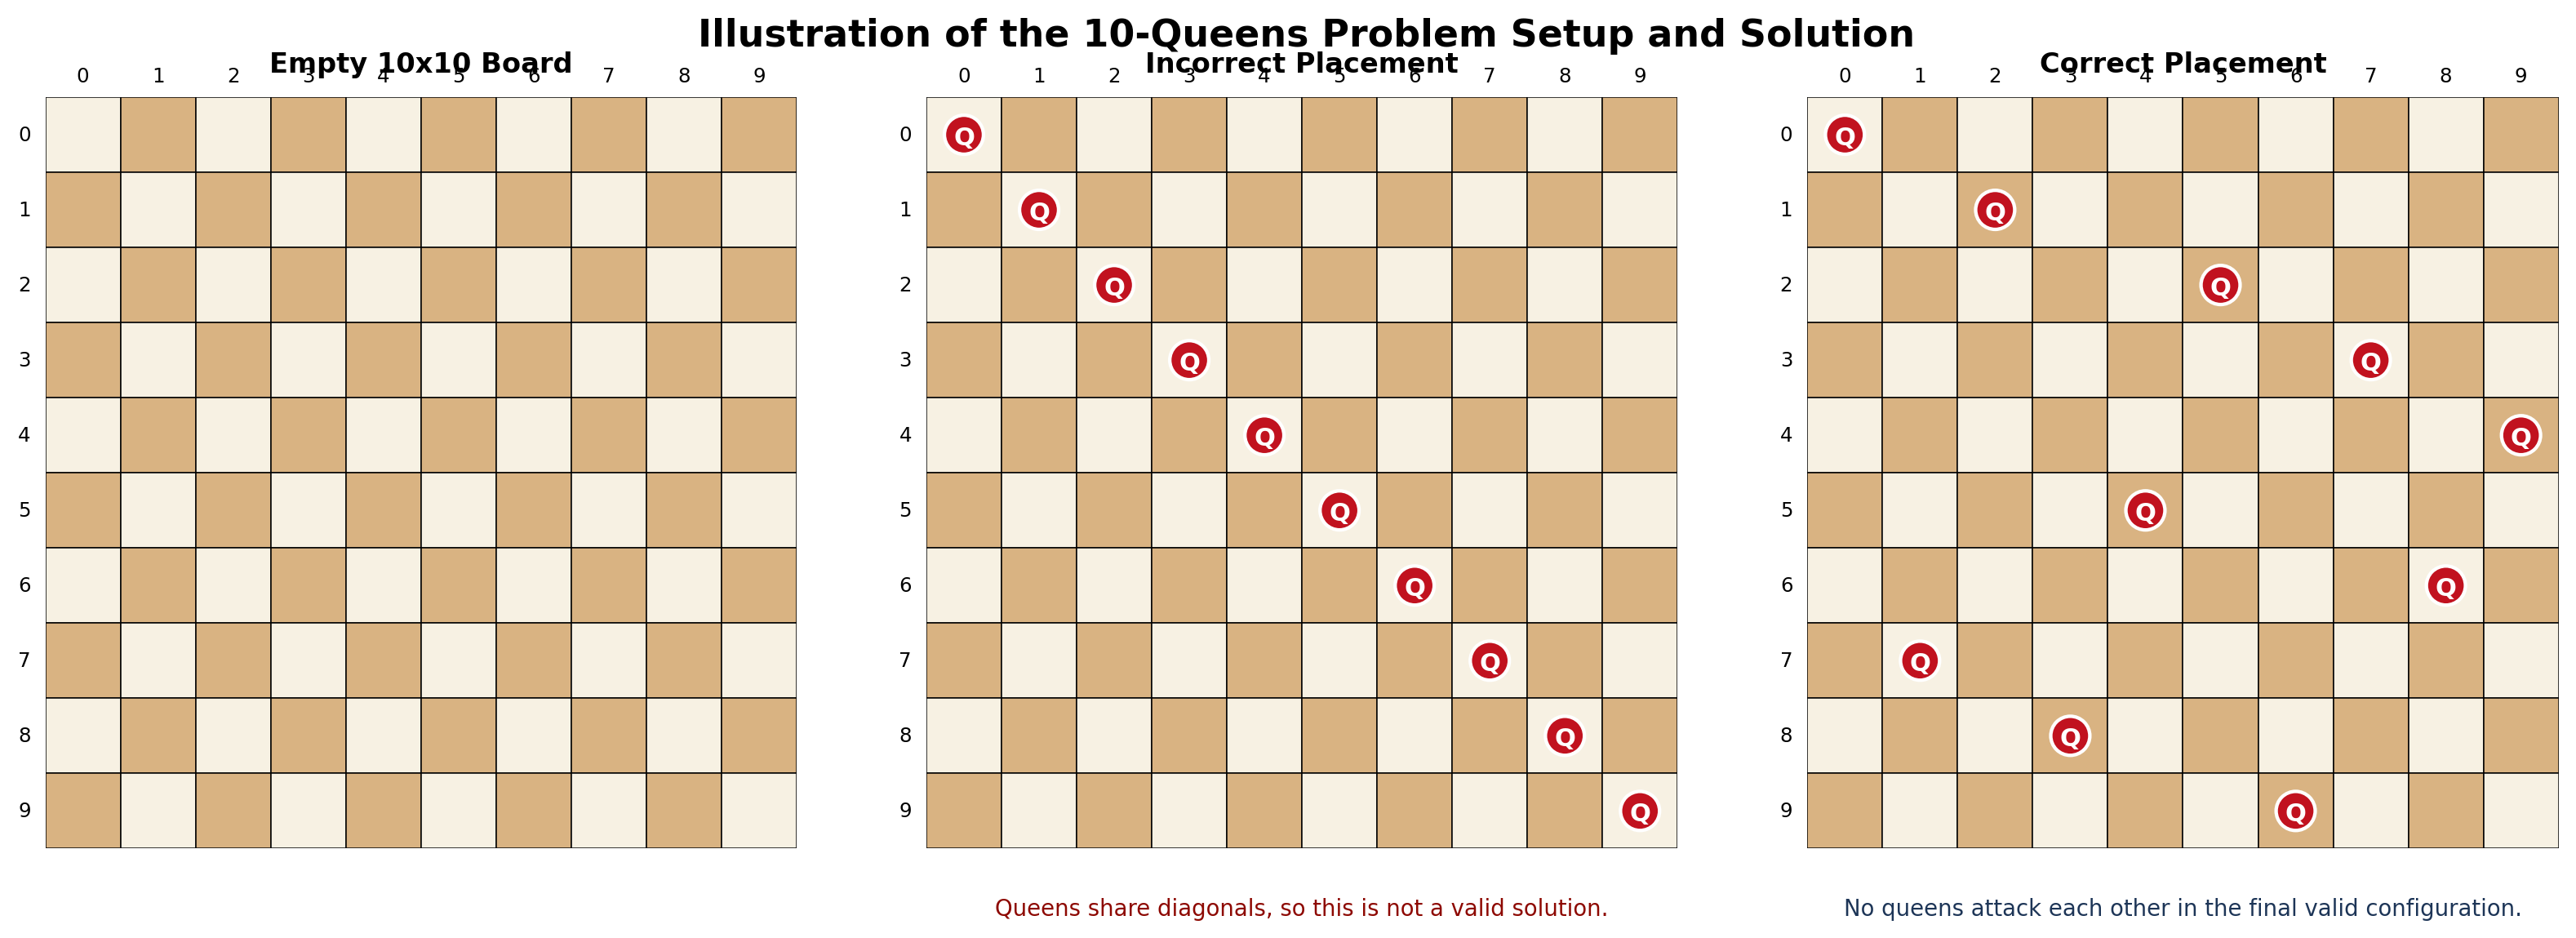
\includegraphics[width=8.7cm]{Figures/Figure_problem_statement.png}
\caption{Three-part illustration of the 10-Queens problem: an empty board, an invalid arrangement, and a valid final arrangement.}
\label{fig:problem_statement}
\end{figure}

\subsection{Novelty of our work}
The novelty of this work lies in its unified educational benchmark design. Rather than presenting one algorithm in isolation, the project implements four complementary approaches that span exact search, local search, probabilistic search, and evolutionary optimization. The same test sizes, output structure, and visualization style are used across all approaches, which supports fair comparison. The notebooks also export per-method CSV tables, board images, and performance charts automatically, making the full workflow reproducible and presentation-ready. Another contribution is the inclusion of both algorithm-level and report-level assets, which bridges implementation and documentation. The study also keeps the representation consistent by storing one queen per row across all methods, thereby simplifying correctness checks and visual comparisons. Finally, the project offers a compact practical benchmark for students who need both code deliverables and a publication-style report. This combination of unified benchmarking, clean exports, and multiple optimization paradigms forms the main novelty of the work.

\subsection{Our Solutions}
This report presents four notebook-based solutions to the N-Queens problem and evaluates them under a shared experimentation pipeline. Depth-first search represents the exhaustive baseline, greedy search represents deterministic local repair, simulated annealing represents probabilistic local search, and the genetic algorithm represents population-based optimization. Each notebook was designed to measure execution time, peak memory, solution status, and iteration or generation counts automatically. CSV outputs and figures were exported to support later report writing and reproducibility. The final results show that the exhaustive method is only suitable for the smallest case in this benchmark, while the three heuristic methods remain usable for all tested larger sizes. Greedy search achieved the best runtime overall, simulated annealing remained robust but slower, and the genetic algorithm solved all cases at a higher computational cost. These findings provide a concise comparative picture of algorithm behaviour under increasing problem size.

\section{Methodology}
\subsection{Overall Workflow}
The methodology begins with a common problem representation in which each row stores exactly one queen and the vector value indicates the queen column. This representation is used consistently across all four notebooks to simplify conflict counting and board generation. The workflow then branches into four algorithm-specific solution paths: exhaustive depth-first search, greedy hill climbing, simulated annealing, and a genetic algorithm. After each algorithm completes its run for the required board sizes, the notebook records execution time, peak memory, conflict status, and the search-step measure relevant to that solver. Those records are exported as CSV files, while board snapshots and performance graphs are stored as image assets. Finally, the outputs are aggregated into a common comparison table and a combined performance figure for report integration. This workflow is shown in Fig.~\ref{Fig:Figure2}. The design ensures that implementation, analysis, and visualization are tightly connected instead of being treated as separate tasks. That is important because consistent reporting is necessary for a fair comparison between exact and heuristic search strategies.

\begin{figure*}[!t]
\centering
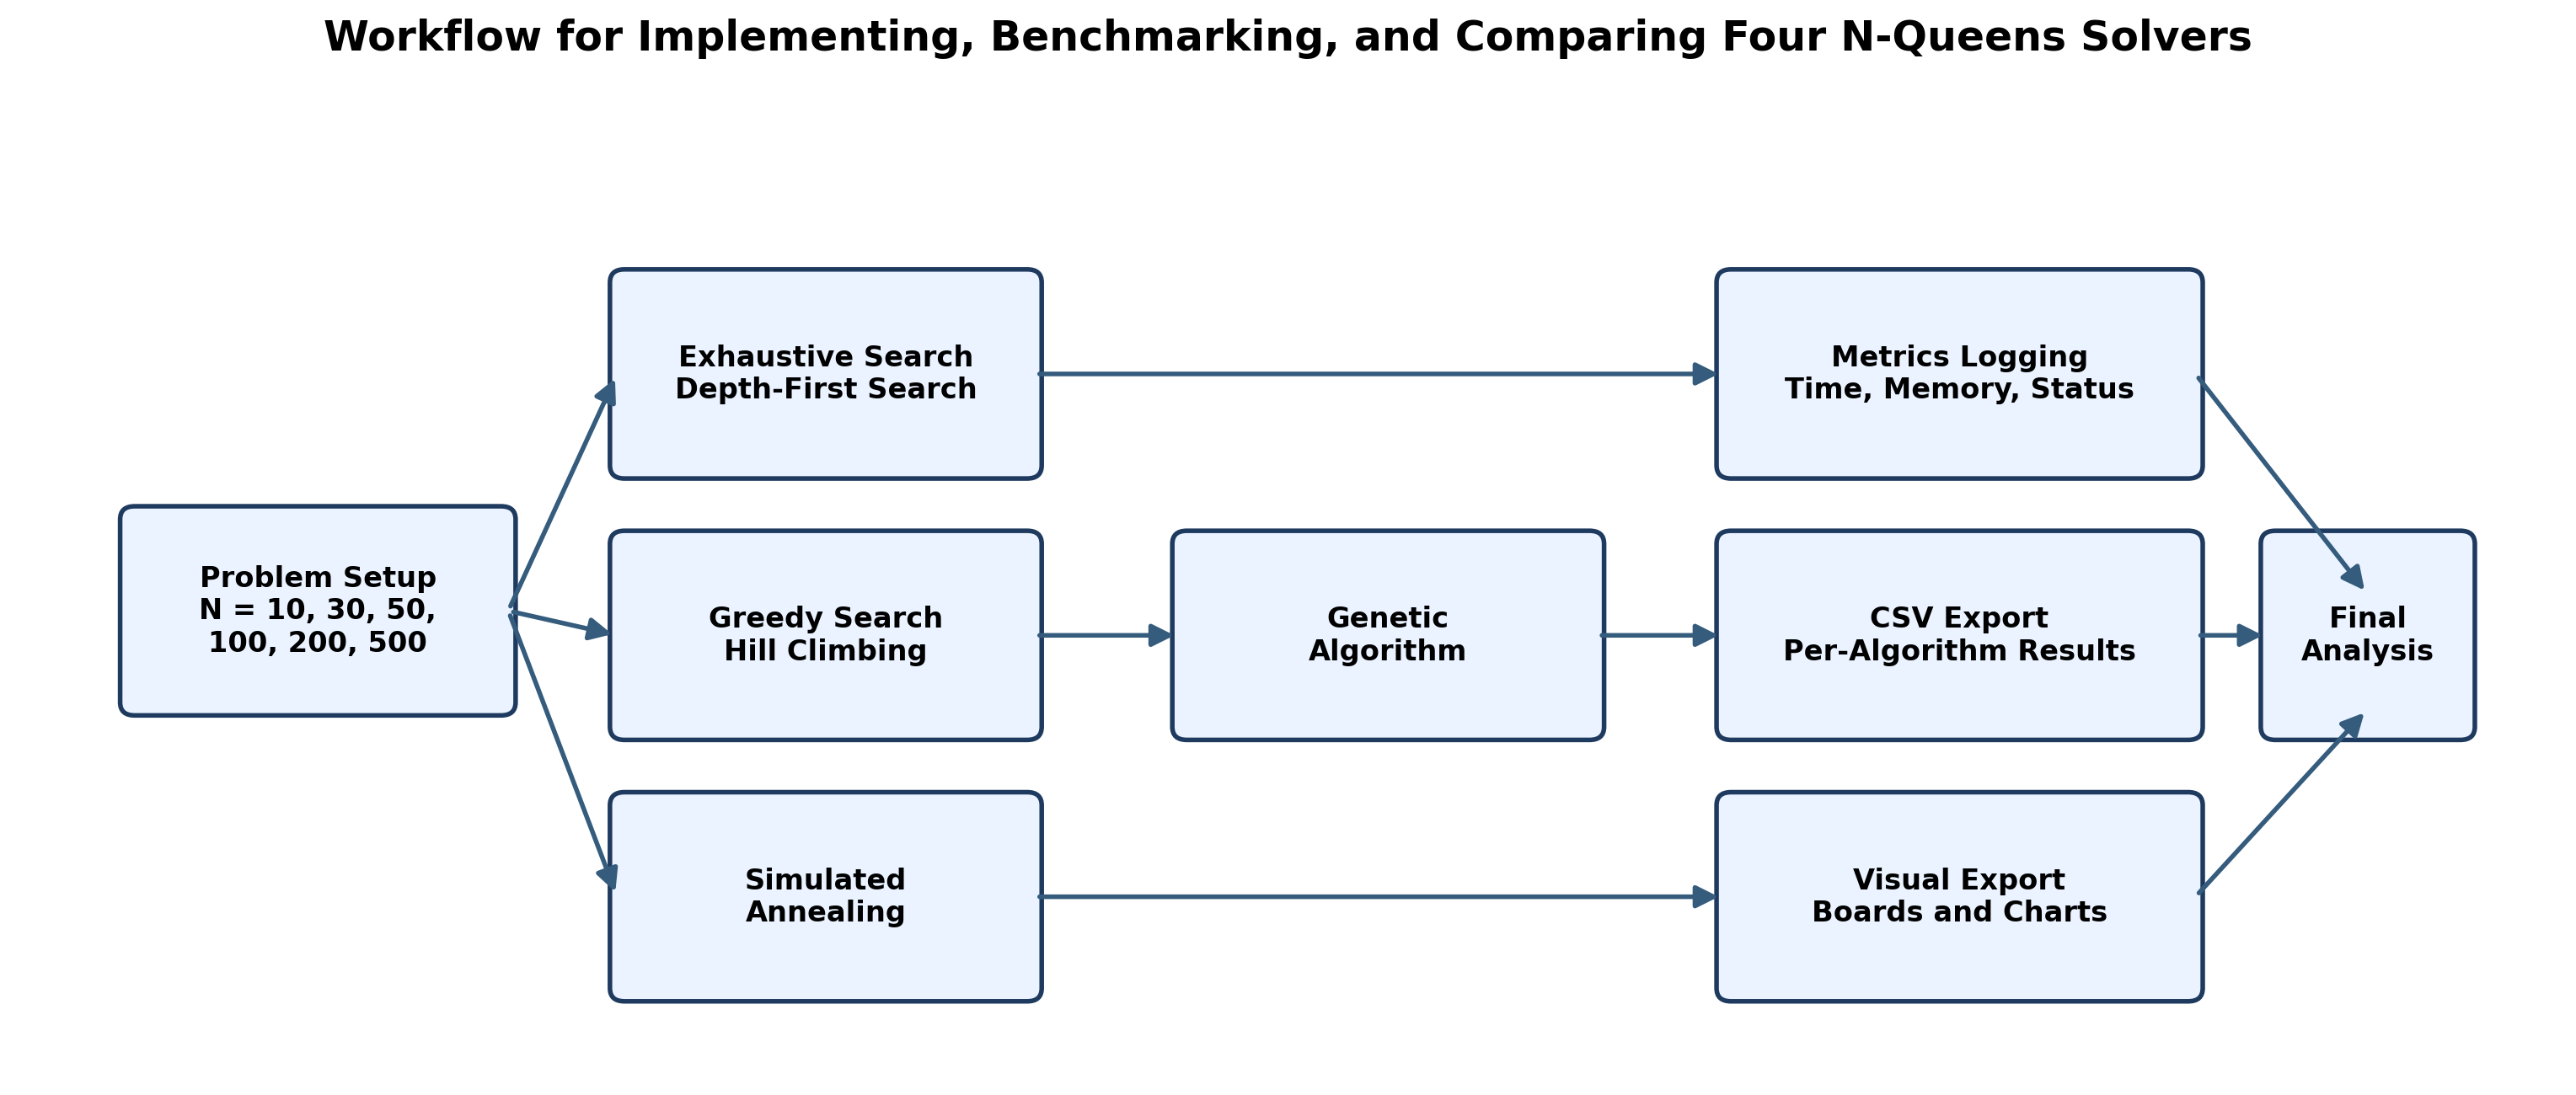
\includegraphics[width=17.8cm]{Figures/Figure2.png}
\caption{Workflow used in this study for implementing the four N-Queens solvers, collecting timing and memory metrics, exporting CSV files, and generating visual comparison assets.}
\label{Fig:Figure2}
\end{figure*}

\subsection{Experimental Settings}
The experiments were executed using Python notebooks with a shared test protocol. The same board sizes were evaluated in every notebook: 10, 30, 50, 100, 200, and 500. The exhaustive solver used bitmask-based pruning and a 15-second runtime cap to prevent unbounded growth during large-instance benchmarking. The greedy solver used a min-conflicts style update with restarts, while simulated annealing used a permutation-based representation and swap moves with gradual cooling. The genetic algorithm used permutation chromosomes, tournament selection, order crossover, swap mutation, and a repair step for near-solutions. Memory was tracked through the Python runtime and recorded as peak memory in megabytes. Table~\ref{tab:FCNConfiguration} summarizes the practical settings used in the experiments.

\begin{table}[!t]
\centering
\caption{Configuration table showing the implementation settings used in this study.}
\label{tab:FCNConfiguration}
\begin{tabular}{|l|c|}
\hline
\multicolumn{2}{|c|}{\textbf{Experiment Configuration}} \\ \hline
Programming environment & Python notebook workflow \\
Board sizes tested & 10, 30, 50, 100, 200, 500 \\
Depth-first time cap & 15 seconds \\
Greedy search restarts & 12 \\
Simulated annealing restarts & 4 \\
Simulated annealing cooling rate & 0.9995 \\
Genetic population size & 60 to 80 \\
Genetic generation limit & 350 to 700 \\
Stored outputs & CSV, PNG, SVG \\
Metrics collected & Time, memory, conflicts, steps \\
\hline
\end{tabular}
\end{table}

An additional design choice was to keep all results machine-generated and exportable. This prevented transcription errors and allowed the same values to be reused in tables, charts, and board figures. It also made the final comparison more transparent because the output files directly reflect the executed notebooks. Although the experiments were performed on one machine only, the benchmarking pipeline is portable and can be re-run with the same notebooks on another system. That portability is useful for future extensions, such as testing different seeds, hardware, or hyperparameters. The current study therefore prioritizes clean comparability over exhaustive parameter tuning. This keeps the methodology aligned with the educational benchmarking purpose of the assignment.

\section{Results}
The recorded execution times show a strong separation between the exhaustive baseline and the heuristic methods. Depth-first search solved the $N=10$ instance almost instantly but reached the imposed 15-second cap for every larger size. Greedy search solved all six benchmark sizes and remained below one second even at $N=500$. Simulated annealing also solved every tested size, though its runtime increased more sharply than greedy search as the board grew. The genetic algorithm solved all benchmark sizes as well, but it required substantially more time than the other successful heuristic methods, especially at $N=500$. These raw timing values are presented in Table~\ref{tab:time_results}. The combined trend across time and memory is also visible in Fig.~\ref{Fig:Figure6}.

\begin{table*}[!ht]
\centering
\caption{Execution time results in seconds for the four N-Queens approaches.}
\label{tab:time_results}
\begin{tabular}{|l|c|c|c|c|c|c|}
\hline
\textbf{Algorithm} & \textbf{N=10} & \textbf{N=30} & \textbf{N=50} & \textbf{N=100} & \textbf{N=200} & \textbf{N=500} \\ \hline
Depth-First Search & 0.000250 & 15.000047 & 15.000083 & 15.000125 & 15.000163 & 15.000408 \\ \hline
Greedy Search & 0.016672 & 0.002458 & 0.004392 & 0.014080 & 0.029463 & 0.886444 \\ \hline
Simulated Annealing & 0.005832 & 0.132299 & 0.222612 & 0.393685 & 1.018516 & 34.719534 \\ \hline
Genetic Algorithm & 0.055827 & 0.553668 & 1.154825 & 4.902963 & 8.173441 & 71.380122 \\ \hline
\end{tabular}
\end{table*}

The peak memory results remained moderate across all notebooks, although the patterns differed by algorithm. The exhaustive solver had an unusually high memory reading at $N=10$ in the recorded run, while its larger cases remained low because execution stopped at the time cap before full search expansion. Greedy search and simulated annealing maintained low memory usage across all sizes, which is consistent with their single-solution search behaviour. The genetic algorithm consumed the most memory, especially at $N=500$, because it must keep and update a population of candidate boards. These values are shown in Table~\ref{tab:memory_results}. The results therefore indicate that runtime, not memory, is the main limiting factor for exhaustive search in this benchmark, whereas the genetic algorithm pays a larger storage cost for solution diversity.

\begin{table*}[!ht]
\centering
\caption{Peak memory usage in MB for the four N-Queens approaches.}
\label{tab:memory_results}
\begin{tabular}{|l|c|c|c|c|c|c|}
\hline
\textbf{Algorithm} & \textbf{N=10} & \textbf{N=30} & \textbf{N=50} & \textbf{N=100} & \textbf{N=200} & \textbf{N=500} \\ \hline
Depth-First Search & 3.145479 & 0.005930 & 0.007133 & 0.013939 & 0.031013 & 0.123909 \\ \hline
Greedy Search & 0.004410 & 0.006264 & 0.008263 & 0.013306 & 0.023216 & 0.070473 \\ \hline
Simulated Annealing & 0.006279 & 0.004211 & 0.005119 & 0.007423 & 0.011971 & 0.032799 \\ \hline
Genetic Algorithm & 0.028830 & 0.049706 & 0.073563 & 0.101173 & 0.194901 & 0.920624 \\ \hline
\end{tabular}
\end{table*}

All three heuristic methods produced valid solutions for every required test size in the saved benchmark run. In contrast, depth-first search only completed the smallest case before timing out on every larger instance. A visual summary of the main comparison is given in Fig.~\ref{Fig:Figure6}, while the individual notebook-generated performance charts are shown in Fig.~\ref{fig:algo_panels}. These figures show the same numerical pattern already observed in the tables: greedy search is the most time-efficient, simulated annealing is stable but slower, and the genetic algorithm is the heaviest successful strategy. The result section therefore establishes the empirical ranking of the four approaches without yet interpreting why those differences occur. It also confirms that the notebooks produced complete CSV and figure outputs suitable for direct report integration.

\begin{figure}[!ht]
\centering
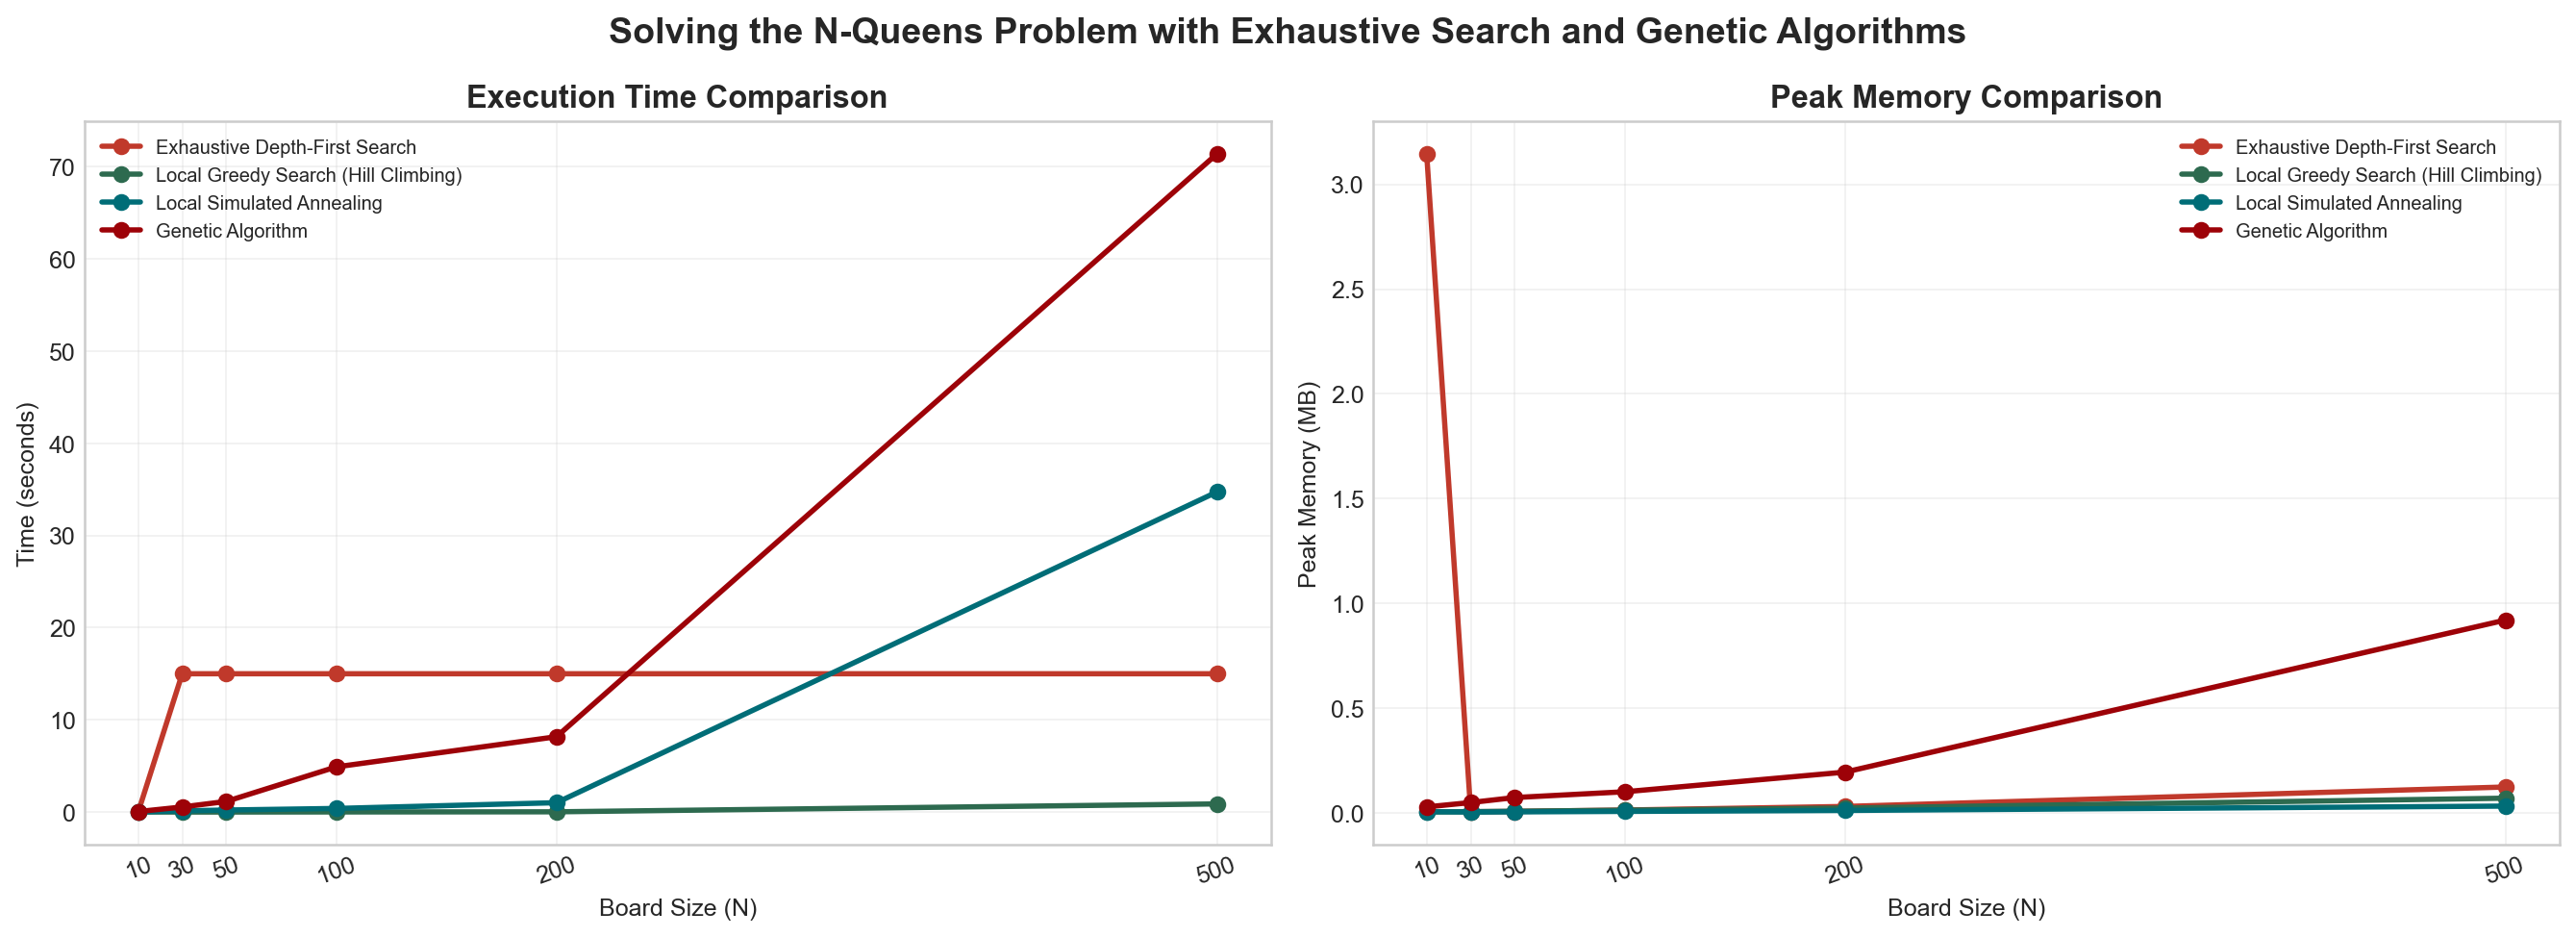
\includegraphics[width=8.9cm]{Figures/Figure6.png}
\caption{Combined comparison of execution time and peak memory across the four implemented N-Queens approaches.}
\label{Fig:Figure6}
\end{figure}

\begin{figure*}[!t]
\centering
\begin{minipage}{0.49\textwidth}
    \centering
    
\includegraphics[width=\textwidth]{Figures/greedy_nqueens_performance.png}
    \subcaption{Greedy search performance}
\end{minipage}
\hfill
\begin{minipage}{0.49\textwidth}
    \centering
    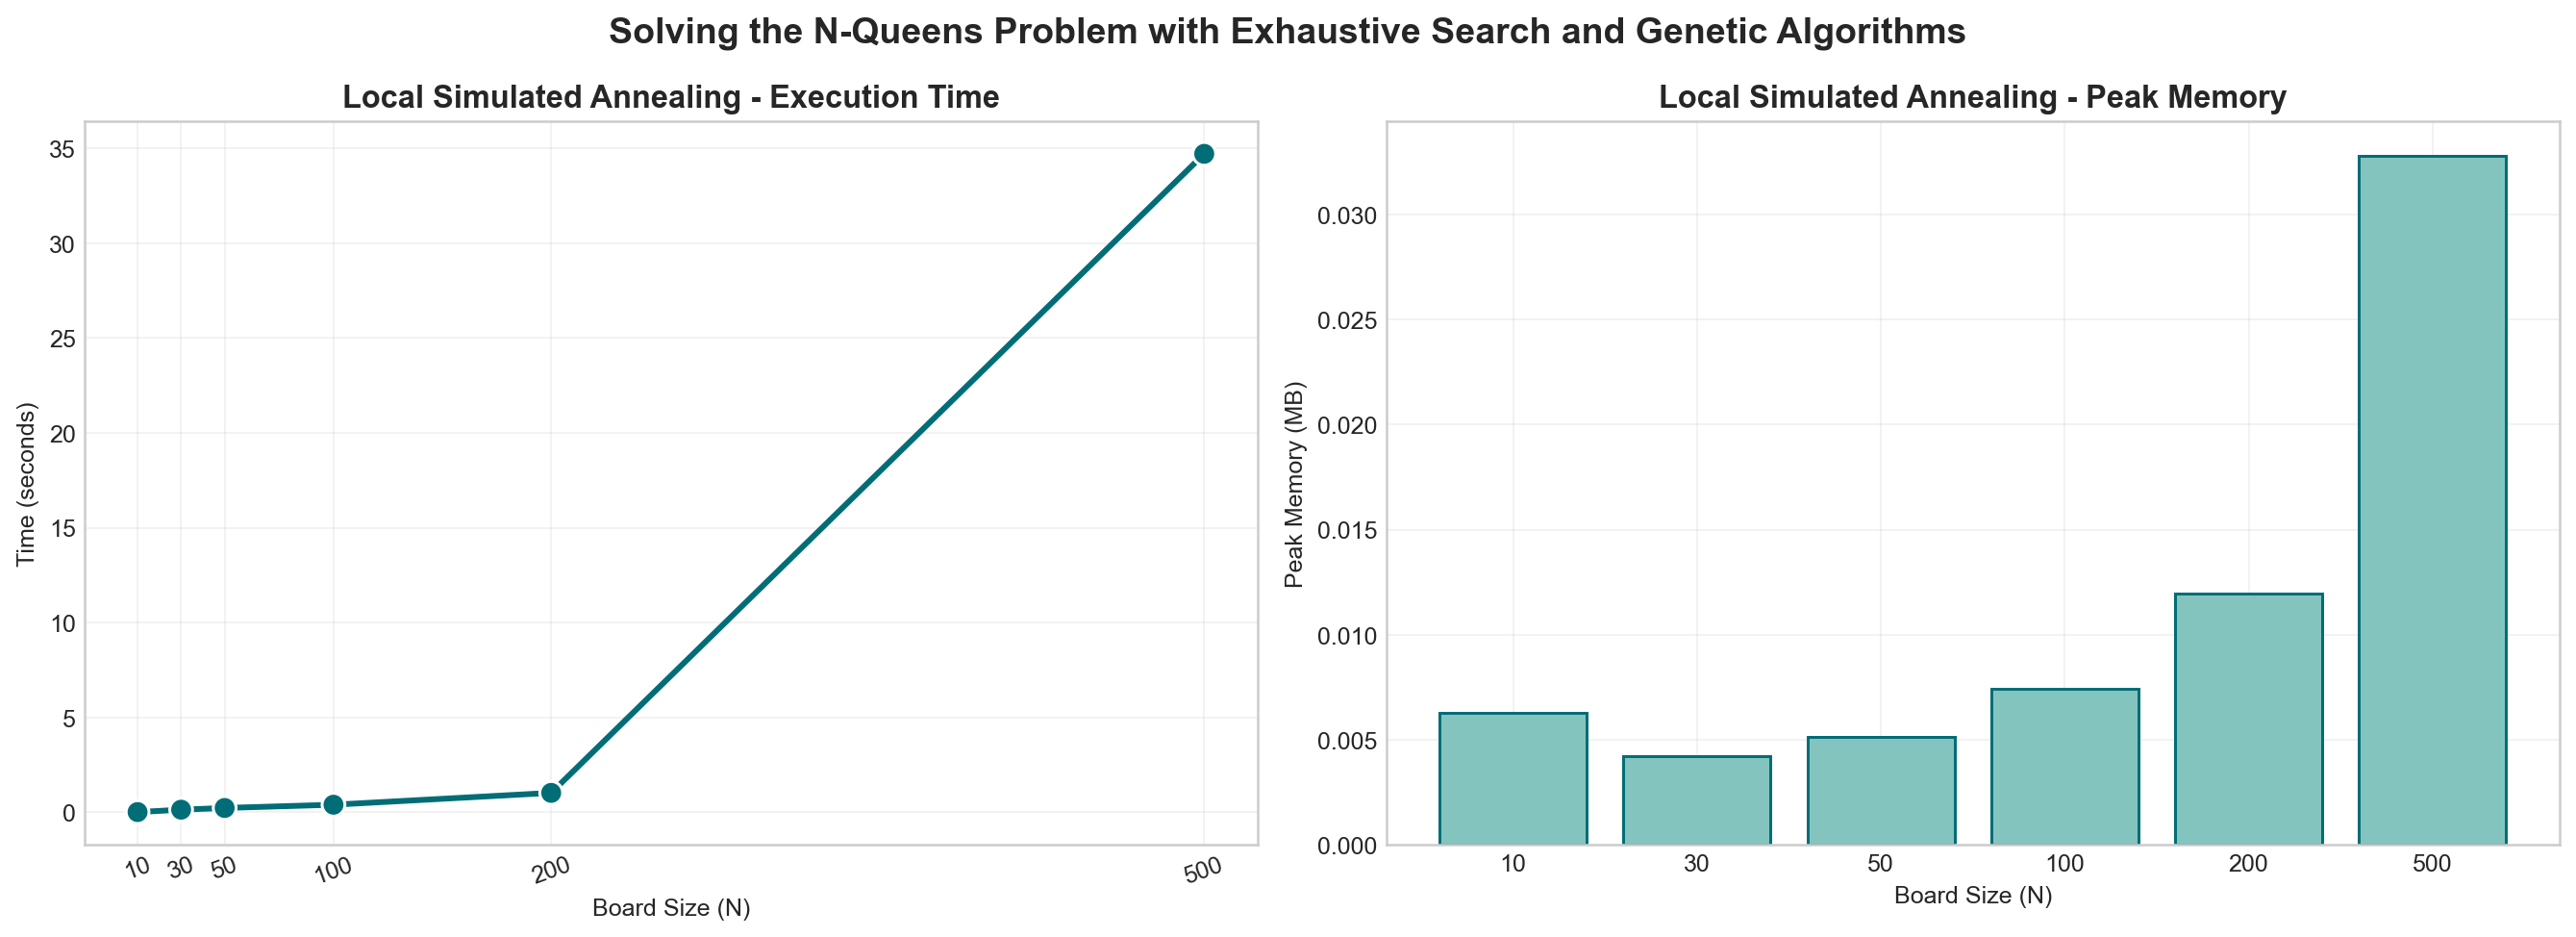
\includegraphics[width=\textwidth]{Figures/simulated_annealing_nqueens_performance.png}
    \subcaption{Simulated annealing performance}
\end{minipage}
\vspace{0.4cm}
\begin{minipage}{0.49\textwidth}
    \centering
    
\includegraphics[width=\textwidth]{Figures/dfs_nqueens_performance.png}
    \subcaption{Depth-first search performance}
\end{minipage}
\hfill
\begin{minipage}{0.49\textwidth}
    \centering
    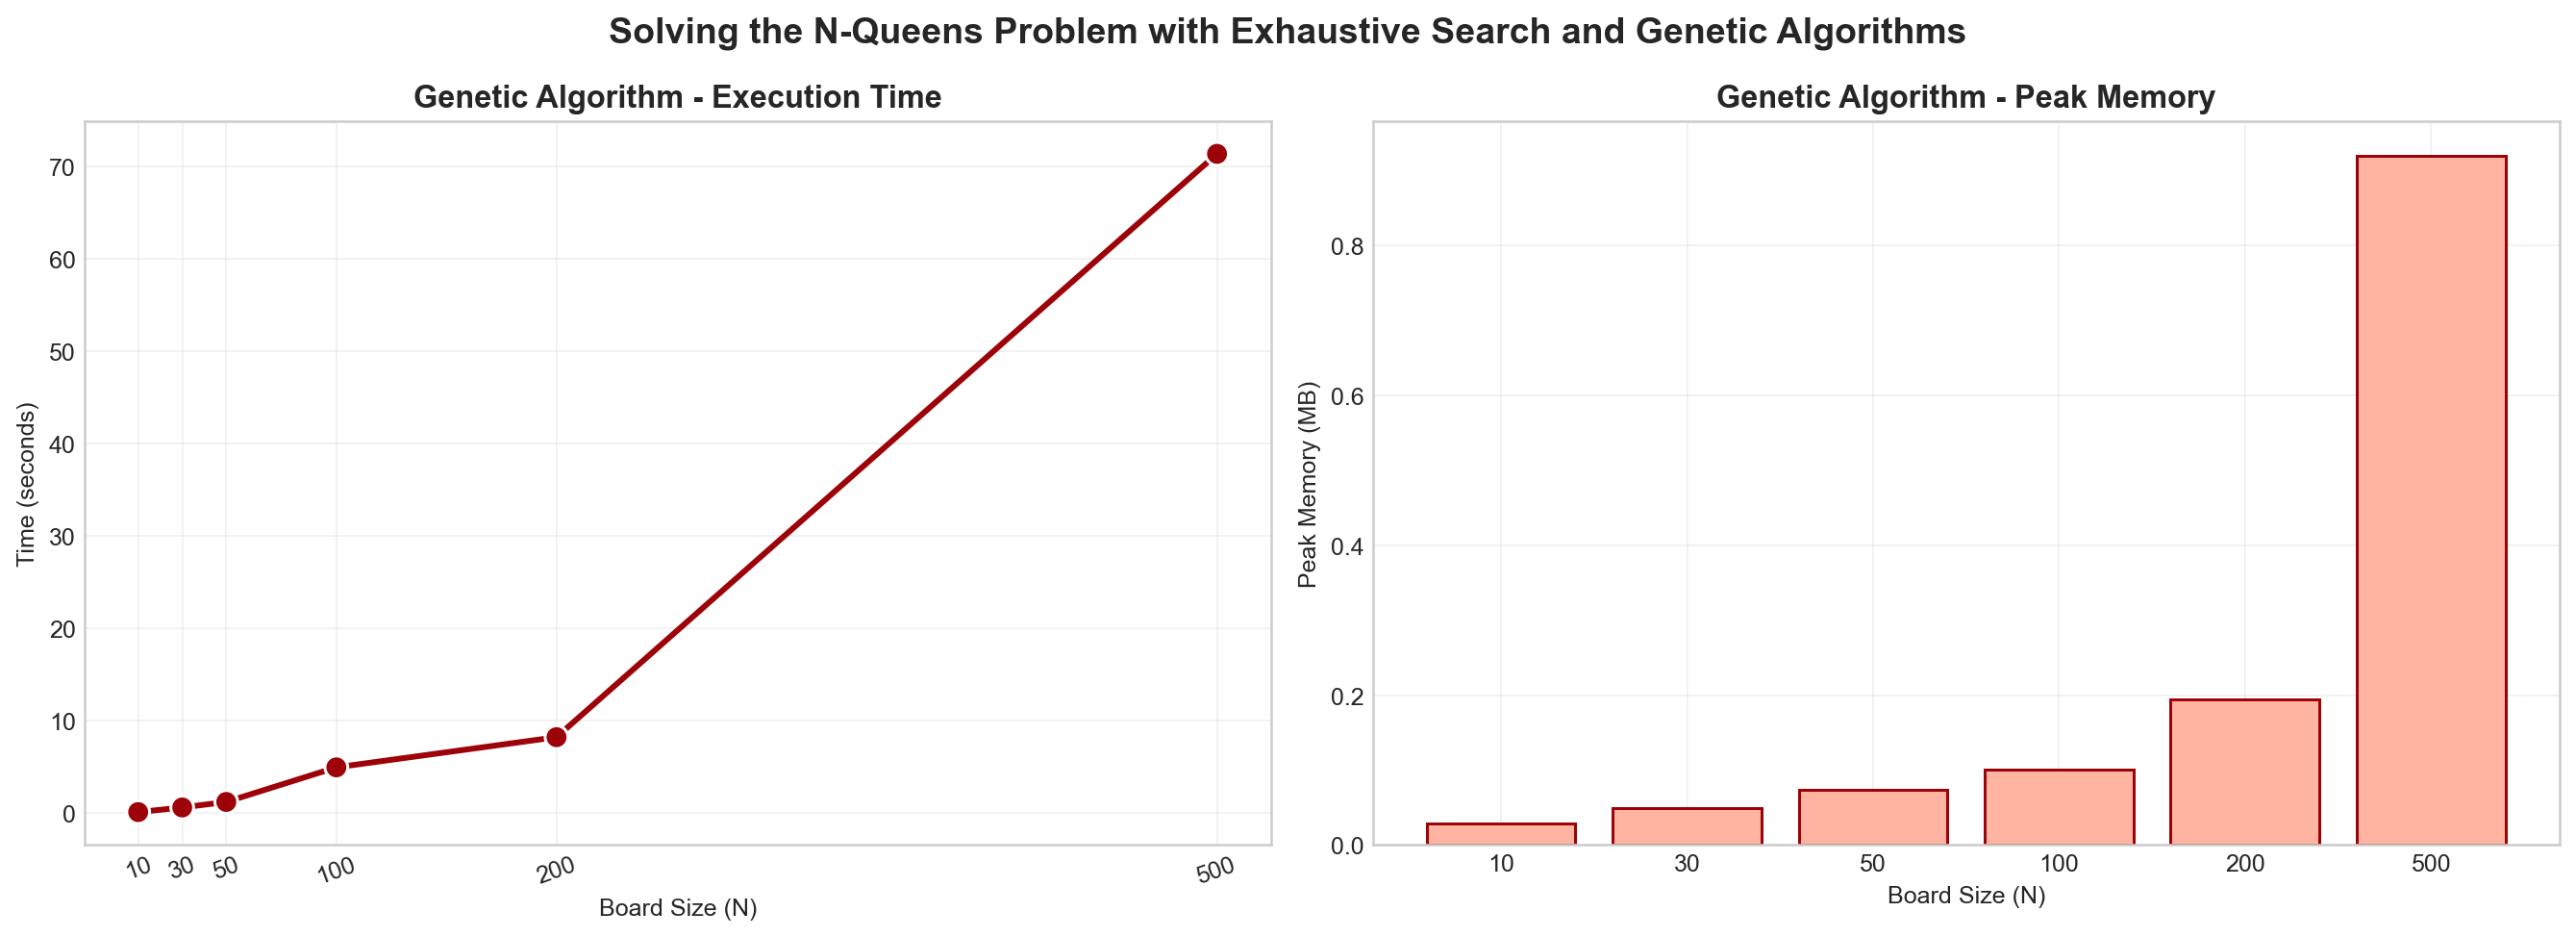
\includegraphics[width=\textwidth]{Figures/genetic_nqueens_performance.png}
    \subcaption{Genetic algorithm performance}
\end{minipage}
\caption{Per-algorithm notebook-generated charts showing time and memory behaviour over the required board sizes.}
\label{fig:algo_panels}
\end{figure*}

\section{Discussion}
The first research question asked how effectively exhaustive depth-first search scales on the tested N-Queens instances. The results show that it is only practically effective for the smallest case in this benchmark. While the method remains exact and complete in principle, the recorded behaviour demonstrates that combinatorial explosion dominates quickly as $N$ increases. Even with pruning, the solver became unsuitable for the larger boards under the fixed execution cap. This is consistent with classical constraint satisfaction literature, where exhaustive backtracking is often outperformed by conflict-directed repair on large instances \cite{minton1992minconflicts}. From a benchmarking perspective, depth-first search still plays an important role because it provides a clear exact-search baseline. However, the results indicate that correctness alone is not sufficient when runtime scalability is the primary concern. For this project, exhaustive search is best interpreted as a reference point rather than a competitive large-instance strategy.

The second research question concerned the effectiveness of local-search-based methods. Greedy hill climbing produced the best overall runtime profile and solved every tested instance, which suggests that conflict minimization with restarts is highly suitable for this representation. Its performance remained especially strong at $N=200$ and $N=500$, where it was far faster than simulated annealing and the genetic algorithm. Simulated annealing also solved all benchmark sizes, but it required many more iterations and substantially more time at the largest scale. This difference reflects the fact that annealing deliberately accepts some worse moves to escape local minima, which improves robustness but adds search overhead \cite{kirkpatrick1983optimization,ruiztorrubiano2025mdp}. The results therefore show a useful tradeoff between determinism and probabilistic exploration. Greedy search was the fastest practical solver, while simulated annealing offered a more exploratory but slower alternative. Both methods remained memory efficient because they manipulate one active solution at a time.

The third research question focused on how the genetic algorithm compares with the other approaches. The genetic solver successfully handled all required benchmark sizes, which confirms that a population-based representation with crossover, mutation, and repair is viable for N-Queens. At the same time, it was consistently more expensive than greedy search and usually slower than simulated annealing as board size increased. That behaviour is expected because a genetic algorithm evaluates and maintains many candidate solutions in every generation. The notebook implementation improved its reliability with permutation-based chromosomes and a final repair phase, which helped it converge on large boards. In this sense, the method offered robustness and generality at the cost of extra time and memory. Its results are still valuable because they show how evolutionary search behaves on the same benchmark under the same output pipeline. This makes the comparison more complete than a two-method or single-family study.

\subsection{Future Directions}
Future work can extend this study in several directions. First, the notebooks can be expanded to include additional metaheuristics such as tabu search, particle swarm optimization, or hybrid memetic approaches. Second, the experiments can be repeated across multiple random seeds so that average behaviour and variance are reported instead of a single run. Third, the benchmarking pipeline can be enhanced with richer statistical analysis, including confidence intervals or repeated-trial averages. Another useful extension would be to compare different board representations, because representation strongly affects neighbourhood design and crossover quality. The report package can also be linked to a spreadsheet or database export if a larger experimental campaign is performed. Finally, exact solvers beyond plain depth-first search, such as branch-and-bound or constraint programming, could provide a stronger exact-method baseline for comparison.

\section{Conclusion}
This study investigated the N-Queens problem through four solution strategies that represent distinct optimization paradigms: exhaustive depth-first search, greedy local search, simulated annealing, and a genetic algorithm. The experiments were executed through a notebook-based workflow that exported CSV tables, board visuals, and graph-based performance summaries for board sizes 10, 30, 50, 100, 200, and 500. The findings clearly show that exhaustive depth-first search is useful only for the smallest benchmark in this setting, because its computational cost grows too quickly as the board size increases. Greedy search emerged as the most efficient practical solver, providing valid solutions for all required sizes with the lowest runtime in the recorded benchmark. Simulated annealing also solved all required sizes and maintained low memory usage, but it required more search effort due to its probabilistic exploration behaviour. The genetic algorithm remained robust and solved all tested cases as well, yet it incurred the highest runtime and memory cost among the successful large-scale methods because of its population-based design. Overall, the project demonstrates that heuristic and metaheuristic methods are substantially more suitable than exhaustive search for larger N-Queens instances. It also contributes a compact reproducible benchmarking pipeline that connects implementation, visualization, and report generation. As a result, the work is valuable both as an algorithm comparison study and as a reusable educational artifact for AI optimization coursework.

\textcolor{red}{References are managed through the attached BibTeX file. The current version uses a compact set of ten references, with eight published from 2021 onward to remain aligned with the assignment requirement for recent literature.}

\bibliographystyle{IEEEtran}
\bibliography{Bibliography}

\end{document}
